%% ------------------------------------------------------------------------- %%
\chapter{Abordagem}
\label{cap:abordagem}


Conforme citado no capítulo~\ref{cap:trabalhos-relacionados}, uma técnica muito utilizada para o problema de \textit{code retrieval} é o \textit{joint embedding}. Para utilizar esta técnica, três fatores devem ser levados em consideração:

\begin{itemize}
    \item Representação de cada palavra de uma sentença ou trecho de código-fonte
    \item Representação da sentença e do trecho de código-fonte
    \item Função objetivo do modelo
\end{itemize}

\section{Representação de cada palavra de uma sentença ou trecho de código-fonte}
\label{sec:abordagem-representacao-token}

As questões e os trechos de código-fonte são compostas por palavras, pontuações, separadores e caracteres de símbolos e operadores matemáticos. Para as questões, que são descritas em linguagem natural, iremos representá-las como um vetor formado por uma sequência de palavaras removendo os caracteres de acento e pontuação.

No caso do código-fonte, iremos partir da  mesma hipótese que utilizamos no artigo \cite{marcelo-vem-2019} apresentado no \acrfull{vem}. Esta hipótese foi levantada por \cite{Allamanis:2018:SML} e diz que software é uma forma de comunicação humana e tem propriedades estatísticas similares a corpora de linguagem natural. A partir disto, iremos aplicar os mesmos procedimentos adotados para as questões aos trechos de código-fonte. Os trechos de código-fonte terão as pontuações e caracteres especiais removidos e serão tratados como uma sequência de palavras.

No nosso caso, tanto as questões e os trechos de código-fonte serão representados por um vetor formado por uma sequência de palavras. E para cada palavra no vetor, devemos definir uma representação.

De acordo com \cite{Goodfellow-et-al-2016:representation-learning}, as redes neurais generalizam bem quando as palavras são representadas através de vetores de representação distribuída. E conforme o próprio \cite{Goodfellow-et-al-2016:representation-learning}, uma boa representação deve auxiliar na aprendizagem de uma tarefa posterior. No nosso caso, as representações devem auxiliar a tarefa de aprender a encontrar uma correlação entre as questões e os trechos de código-fonte mais relevantes.

Neste trabalho, cada palavra será representada através de um vetor de representação distribuída. Para mapear as palavras para vetores de representação distribuída, utilizaremos inicialmente o algoritmo não-supervisionado \textit{word2vec}. Utilizaremos o \textit{word2vec} com \textit{skip-gram}. O \textit{skip-gram} prediz as palavras do contexto a partir de uma palavra alvo. Diferente do CBoW que prediz a palavra alvo a partir das palavras do contexto. 

Segundo \cite{mikolov2013distributed}, \textit{skip-gram} obteve um desempenho melhor em problemas semânticos, e.g., relacionar uma palavra masculina com a equivalente feminina, relacionar o nome de uma capital a um país ou cidade a um estado. No caso do código-fonte, isto é uma característica importante, pois pode ajudar a agrupar os \textit{tokens} de acordo com o tipo. Por exemplo, agrupar a instrução de decisão \textit{while} próxima da instrução \textit{for}. E relacionar a instrução de decisão \textit{if} próxima da \textit{else}.

O \textit{word2vec} irá mapear cada palavra para um espaço vetorial $\mathbb{R}^{d}$. Seja $\mathbb{Q}$ o conjunto de palavras das questões, e $\mathbb{C}$ o conjunto de palavras presentes nos trechos de código-fonte. Para cada palavra ${q} \in \mathbb{Q}$ e ${c} \in \mathbb{C}$, teremos:

\begin{equation}
    f: {q} \rightarrow t_{q}, t_{q} \in \mathbb{R}^{d}
\end{equation}

\begin{equation}
    g: {c} \rightarrow t_{c}, t_{c} \in \mathbb{R}^{d}
\end{equation}
Onde $f$ e $g$ são o \textit{word2vec} com o algoritmo \textit{skip-gram}. $f$ e $g$ irão mapear cada palavra pertencente a um vocabulário a uma matriz distinta $\bm{T_{q}}$ e $\bm{T_{c}}$.
Teremos duas matrizes: $\bm{T}_{q}^{|\mathbb{Q}| X d}$ e outra $\bm{T}_{c}^{|\mathbb{C}| X d}$, onde $|\mathbb{Q}|$ e $|\mathbb{C}|$ são o tamanho do vocabulário das questões e trechos de código-fonte, respectivamente. E $d$ é a dimensão do vetor de representação distribuída.

\section{Representação da sentença e do trecho de código-fonte}

Com cada palavra representada por um vetor de representação distribuída, o próximo passo é combiná-las para obter uma representação para a questão e o trecho de código-fonte. Para isto, a nossa proposta é utilizar uma arquitetura CNN. 

Para cada sentença (e.g. questão ou trecho de código-fonte), seja $\bm{x}(i) \in \mathbb{R}^{d}$ um vetor de representação distribuída para $i^{th}$ palavra da sentença, onde $d$ é a dimensão do vetor. Dado que uma sentença tem $n$ palavras, temos que $\bm{x}$ pode ser escrito da seguinte maneira: $\bm{x} = \{ \bm{x}(1), \bm{x}(2), . . ., \bm{x}(n) \}$.

Seja $\bm{x}(i, i + j)$ referência a concatenação dos vetores $\bm{x}(i), \bm{x}(i + 1), . . ., \bm{x}(i + j)$. A operação de convolução é aplicada a este vetor. Isto envolve um filtro convolucional $\bm{F}  = [\bm{F}(1),· · ·, \bm{F}(m)]$, tal que $\bm{F} \in \mathbb{R}^{m X d}$. Este filtro é aplicado a uma janela de $m$ palavaras para produzir um novo vetor. Por exemplo, um novo vetor $\bm{c}(i)$, utilizando a seguinte janela de palavras $\bm{x}(i, i + m - 1)$, é calculado da seguinte maneira:

\begin{equation}
    \bm{c}(i) = tanh \left[\left(\sum_{j=i}^{i + m - 1} \bm{x}(j)^{T}\bm{F}(j)\right) + b\right]
\end{equation}

onde $b$ é o \textit{bias} e $\bm{F}$ e $b$ são parâmetros do filtro. As figuras~\ref{fig:first-step-convolutional}, \ref{fig:second-step-convolutional} abaixo ilustram um exemplo dos dois primeiros passos da aplicação de um filtro convolucional $\bm{F} \in \mathbb{R}^{m X d}$, onde $m = 2$ e $d = 5$. Este filtro é aplicado a uma sentença formado por 6 palavras, que é representado pelo vetor de representação distribuída $\bm{x} \in \mathbb{R}^{n X d}$, onde $n = 6$ e $d = 5$. Pelas figuras, podemos perceber que o parâmetro $m$ do filtro $\bm{F}$ define como as palavras são combinadas. Neste caso, foram combinadas de duas em duas, um bi-gram.

\begin{figure}[h]
    \centering
    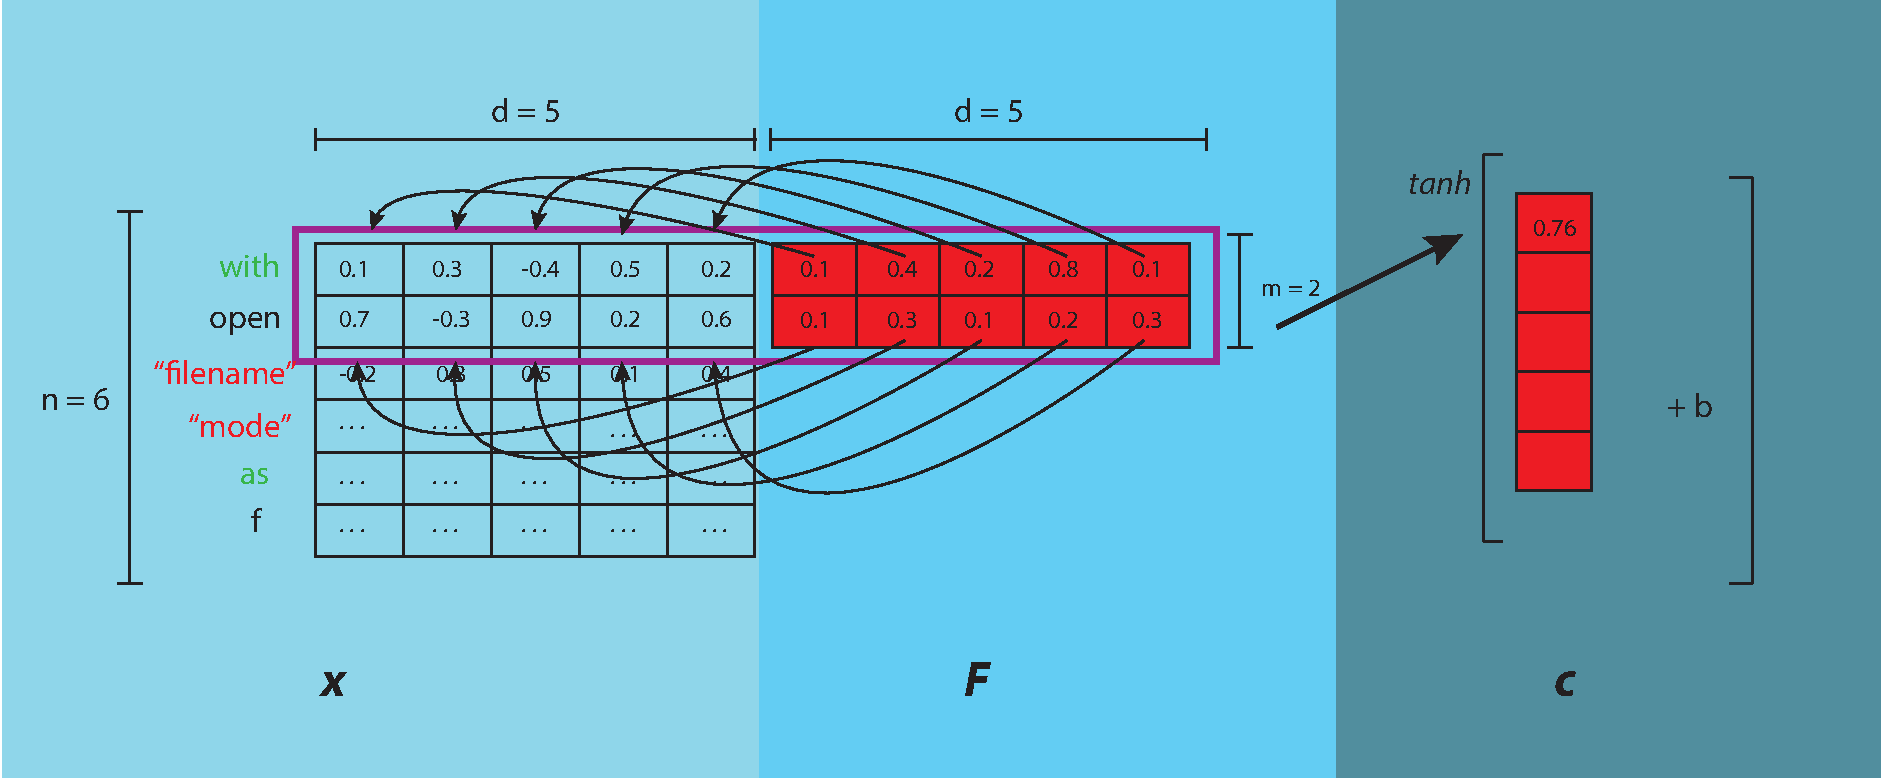
\includegraphics[width=1\textwidth]{figuras/cap-problema/first-step-convolution.pdf}
    \caption{Primeiro passo de um filtro convolucional F.}
    \label{fig:first-step-convolutional}
\end{figure}

\begin{figure}[h]
    \centering
    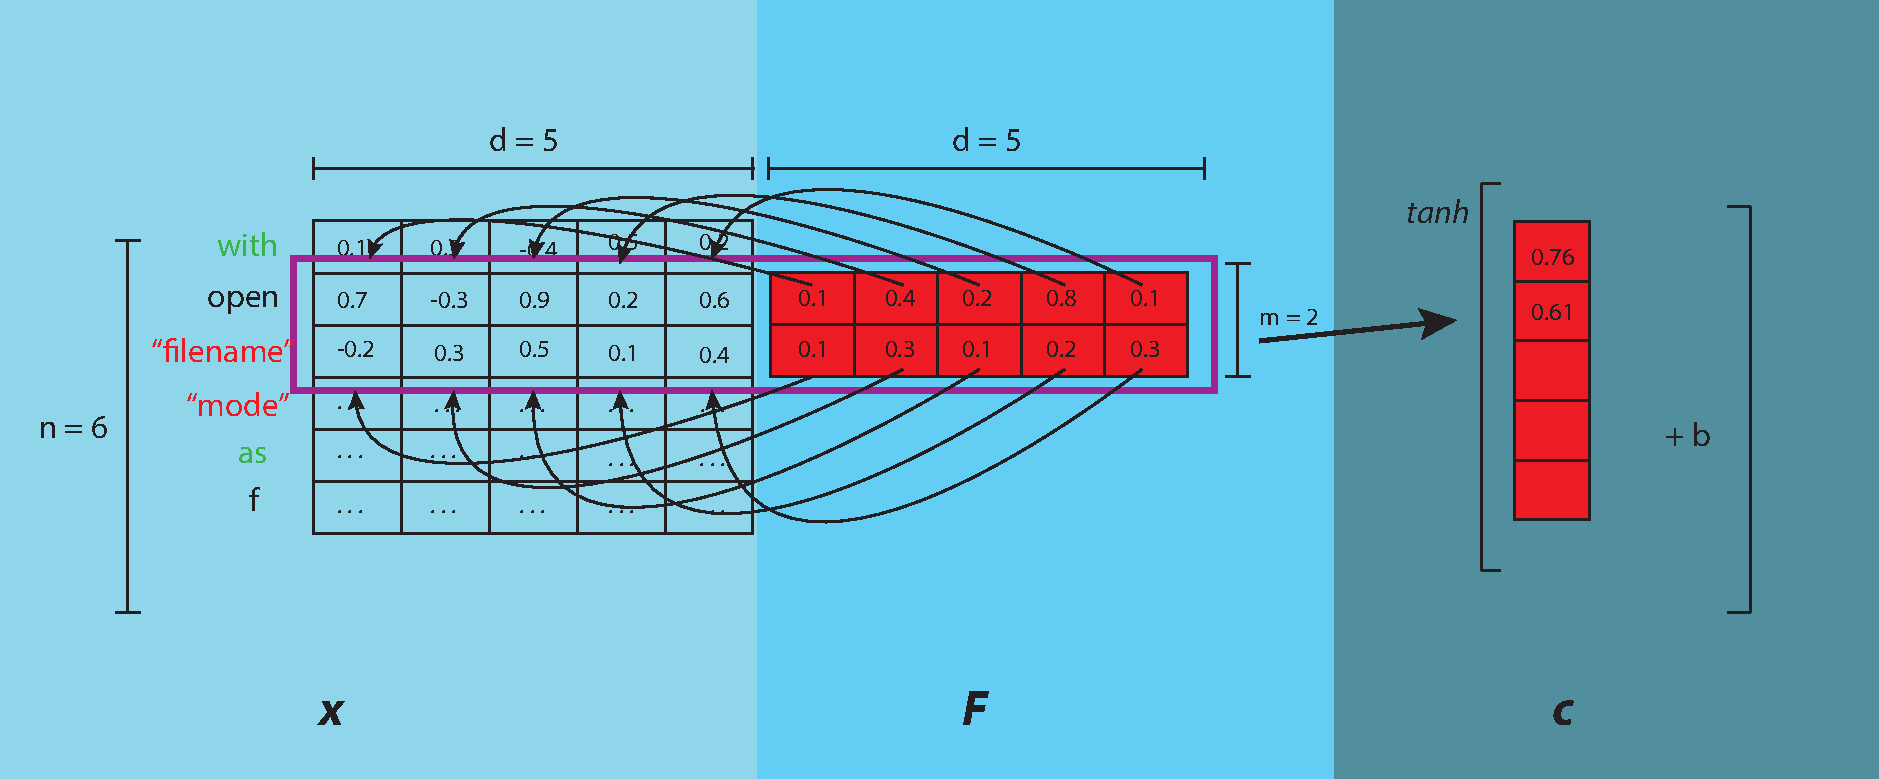
\includegraphics[width=1\textwidth]{figuras/cap-problema/second-step-convolution.pdf}
    \caption{Segundo passo de um filtro convolucional F.}
    \label{fig:second-step-convolutional}
\end{figure}


O filtro $\bm{F}$ é aplicado a todas possíveis janelas de palavras utilizando os mesmos pesos para produzir um mapa das características (\textit{feature map}).

\begin{equation}
    \bm{c} = \{ \bm{c}(1), \bm{c}(2), . . ., \bm{c}(n - m + 1) \} 
\end{equation}




Em uma arquitetura CNN, existem centenas de filtros convolucionais $\bm{F}$, também chamados de \textit{kernel}, de diferentes tamanhos $m$ que percorrem toda uma sentença $\bm{x}$. Cada \textit{kernel} extrai características específicas de n-gram. Após a camada convolucional, i.e., após o cálculo do vetor $\bm{c}$, normalmente uma camada de maxpool é aplicada. Esta camada reduz a dimensionalidade do vetor de entrada aplicando uma operação \textit{max}, que extrai o maior elemento de cada vetor.

\begin{equation}
    \bm{c'} = max\{\bm{c}\}
\end{equation}


Esta redução da dimensionalidade é um fator importante para problemas de classificação, por exemplo. Independente do tamanho da entrada e do filtro, a dimensão da camada de saída vai ser mantida. Além disso, a camada \textit{maxpool} é invariante a pequenas translações. Isto permite extrair características relevantes (e.g. palavras referindo-se a leitura de arquivo: \emph{file} e \emph{open}) de uma sentença independente da sua localização e adiciona-las na representação final \citep{tom-young:trends-deep-learning-nlp}.

A figura abaixo ilustra um exemplo da aplicação de diferentes filtros convolucionais com diferentes tamanhos de janela $m$ em uma sentença de 6 palavras. A sentença é representada através de um vetor $\bm{x} \in \mathbb{R}^{n X d}$, onde $n = 6$ e $d = 5$. Para um vetor $\bm{x} = \{\bm{x}(1), \bm{x}(2), . . ., \bm{x}(n) \}$, $\bm{x}(i) \in \mathbb{R}^{d}, 1 \leq i \leq n$ é um vetor de representação distribuída e representa a $i^{th}$ palavra da sentença. Neste exemplo, temos 3 filtros $\bm{F} \in \mathbb{R}^{m x d}$, onde $d = 5$ e $m$ varia para cada um. Neste caso, os valores de $m$ são $2$, $3$ e $4$. Cada filtro tem tamanho $f = 2$, totalizando 6 filtros que são aplicados ao vetor $\bm{x}$, ao final.

\begin{figure}[h]
    \centering
    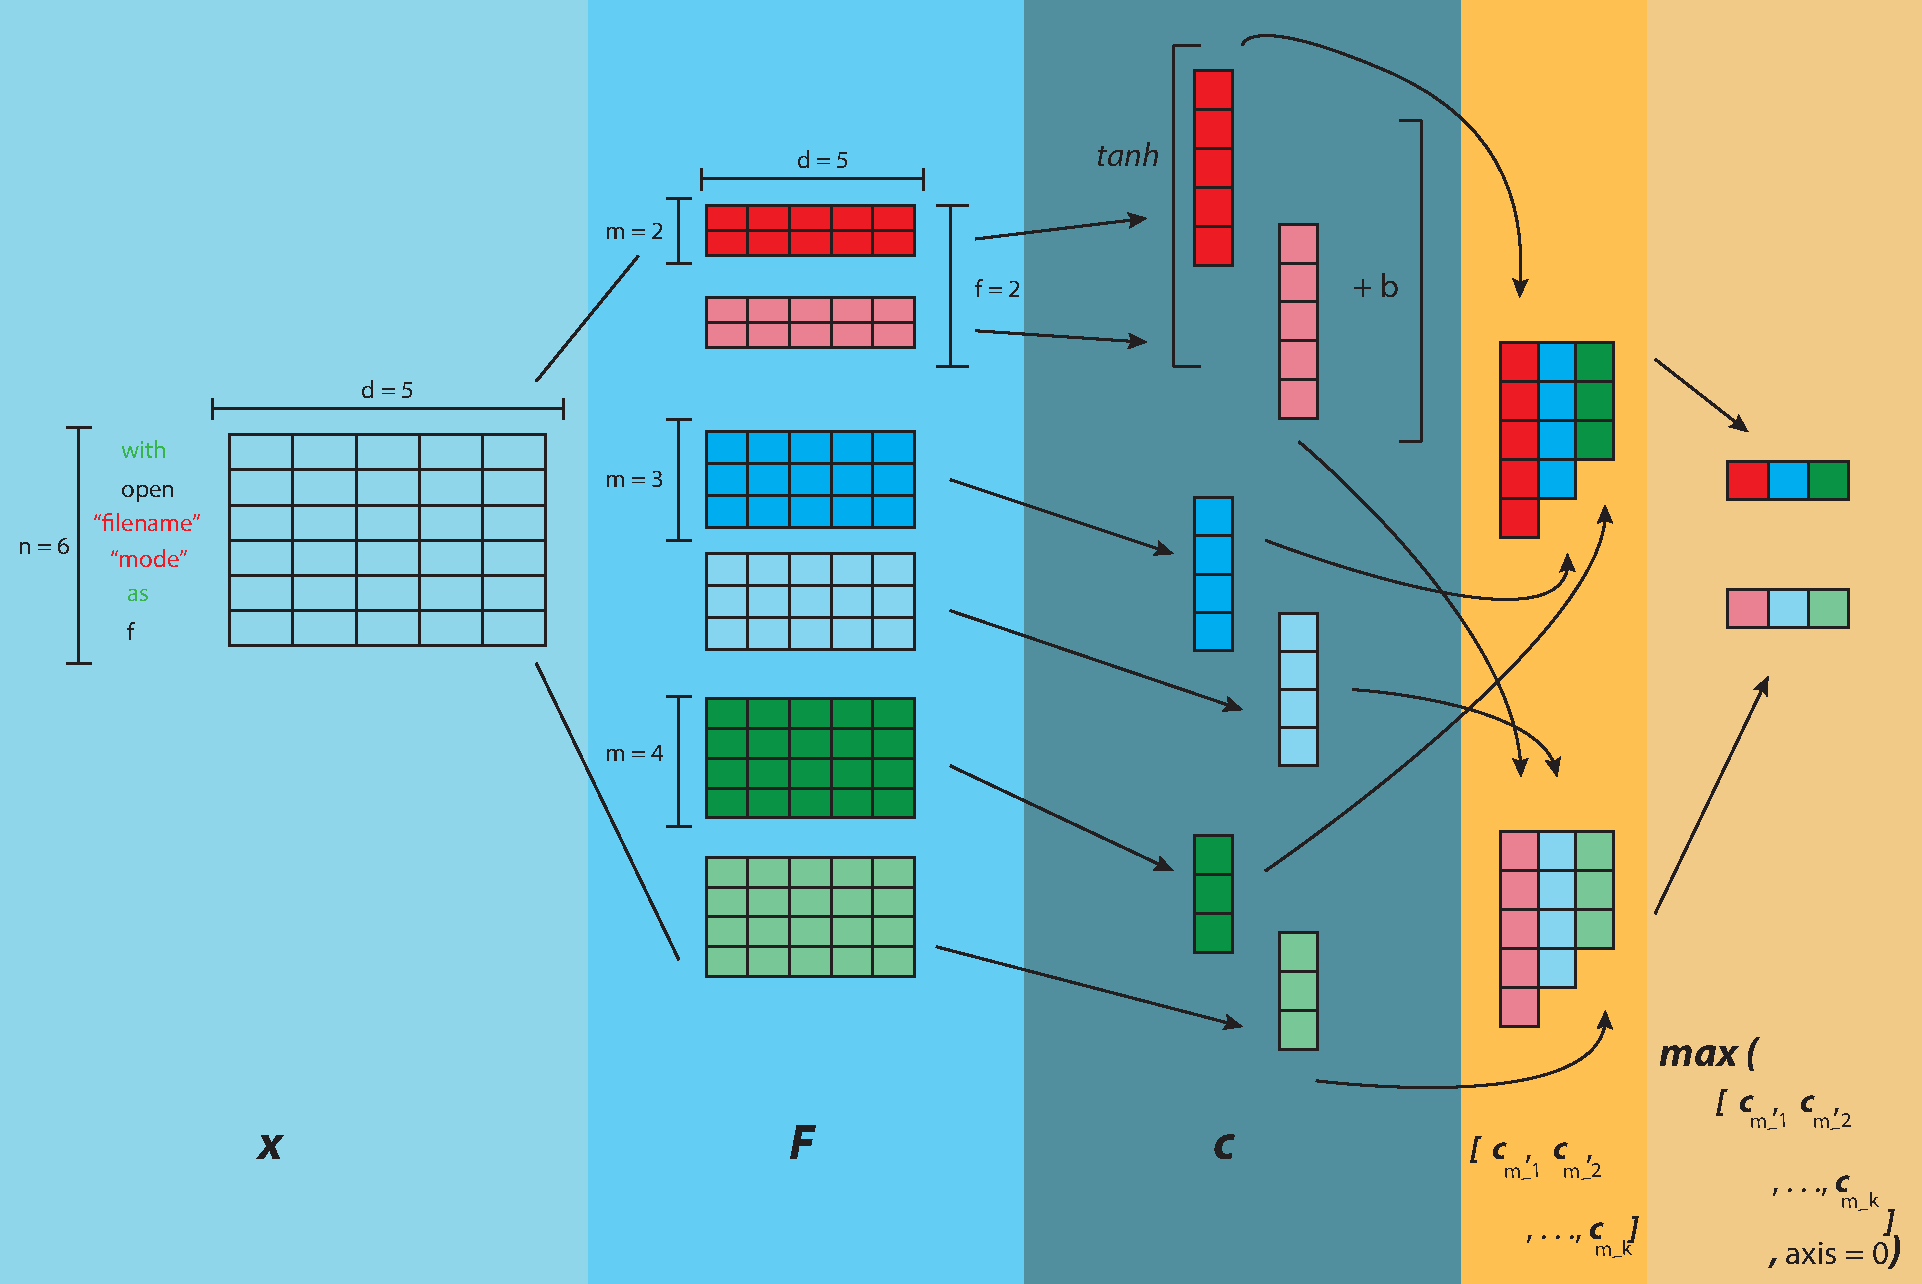
\includegraphics[width=1\textwidth]{figuras/cap-problema/cnn-architecture.pdf}
    \caption{Arquitetura proposta.}
    \label{fig:cnn-architecture-proposal}
\end{figure}

Conforme a figura, após a operação de convolução, i.e., o cálculo de $\bm{c}$, realizamos a concatenação dos vetores de saída de diferentes tamanhos de janela $m$. Pois cada filtro gera um vetor $\bm{c}$ diferente. O filtro $\bm{F}_{1}$ de tamanho de janela $m_1$ gera um vetor $\bm{c}_{m_1}$. O filtro $\bm{F_2}$ de janela $m_2$ gera um vetor $\bm{c}_{m_2}$. E assim por diante.

\begin{equation}
    \bm{c}_{\bm{m}} = \left[\bm{c}_{m_1}, \bm{c}_{m_2}, . . ., \bm{c}_{m_{k}}\right]
\end{equation}

Onde $\bm{c}_{\bm{m}}$ é o resultado da concatenação dos diferentes vetores $\bm{c}$, $\bm{m}$ é um vetor com os diferentes tamanhos de janela, $\bm{m} = \{m_1, m_2, . . ., m_{k}\}$, e $k$ é a quantidade de elementos. No nosso exemplo, $\bm{m} = \{2, 3, 4\}$ e $k = 3$. Somente ao final que aplicamos a camada \textit{maxpool}. A camada \textit{maxpool} aplica a operação \textit{max}, obtendo o vetor de representação final da sentença $\bm{c'}_{\bm{m}}$. Conforme a ilustração, a operação \textit{max} é aplicada no eixo $0$, portanto o vetor final $\bm{c'}_{\bm{m}}$ é obtido da seguinte maneira:

\begin{equation}
    \bm{c'}_{\bm{m}} = max\left(\left[\bm{c}_{m_1}, \bm{c}_{m_2}, . . ., \bm{c}_{m_k}\right], axis = 0\right)
\end{equation}

Onde $axis$ define ao longo de qual eixo a função será aplicada. De forma equivalente, $\bm{c'}_{\bm{m}}$ poderia ser calculado do seguinte modo:

\begin{equation}
    \bm{c'}_{\bm{m}} = \left[max(\bm{c}_{m_1}), max(\bm{c}_{m_2}), . . ., max(\bm{c}_{m_k})\right]
\end{equation}

Neste caso, $\bm{c'}_{\bm{m}}$ será o vetor de representação final da nossa sentença. No nosso trabalho, a sentença pode ser tanto uma questão quanto um trecho de código-fonte. O próximo passo é definir uma função objetivo que induza o nosso modelo a mapear estes vetores em um espaço vetorial, de tal forma que os vetores de representação de uma questão fiquem próximos dos vetores de trechos de código anotados como solução.


\section{Função objetivo}
\label{sec:funcao-objetivo}

Tanto o bi-LSTM com CNN e o CNN geram representações para as questões e os trechos de código-fonte. O intuito é encontrar um modelo que correlacione as questões as respostas em um mesmo espaço vetorial. Neste trabalho adotaremos a mesma abordagem utilizada por \cite{feng-2015}, o método \textit{pairwise}. O método \textit{pairwise} consiste em treinar o modelo para classificar as respostas corretas com uma pontuação maior do que as incorretas. Formalmente, o modelo será treinado do seguinte modo:

Seja $\mathbb{Q}$ um conjunto de questões e $\mathbb{C}$ um conjunto dos trechos de código-fonte. $\mathbb{Q}$ e $\mathbb{C}$ compõem o conjunto de dados de treinamento.

Dado uma tripla $<q, c^{+}, c^{-}>$, onde $c^{+}$ é uma resposta correta observada para a questão $q \in \mathbb{Q}$. E $c^{-}$ é uma resposta incorreta. A função de custo \textit{hinge} é definida como:

\begin{equation}
J = max(0, m - h_{\theta}(q, c^{+}) + h_{\theta}(q, c^{-}))
\end{equation}

Onde $m$ é uma margem e $h_{\theta}$ é uma função de similaridade, e.g., \textit{cosine}. O objetivo é minimizar a função $J$. Para isto, o modelo vai ser incentivado a satisfazer a seguinte condição: $h_{\theta}(q, c^{+}) - h_{\theta}(q, c^{-}) \geq m$. Quer dizer, a função \textit{hinge} induz o modelo a classificar as respostas corretas com uma pontuação maior do que as incorretas por uma certa margem $m$.


\section{Considerações}

As redes convolucionais partem da hipótese de que a função que a camada deve aprender contém apenas interações locais e são invariantes a pequenas translações. Esta invariância é também uma característica da camada \textit{maxpool}. Para problemas NLP, o CNN tenta extrair as características mais importantes de uma sentença. No caso do trecho de código-fonte, a identificação da interação local entre as palavras pode auxiliar na obtenção de uma representação contextualizada. Para inferir o contexto do trecho de código a seguir, o CNN deveria ser capaz de identificar a interação entre as palavras \emph{csv} e \emph{writer} na linha 4, por exemplo. 

\begin{mypython-linenumber}{CNN}
import csv

with |\colorbox{green}{open}|("output.csv", "wb") as f:
    writer = |\colorbox{green}{csv}|.|\colorbox{green}{writer}|(f)
    writer.|\colorbox{green}{writerows}|(a)
\end{mypython-linenumber}
\todo{colocar um caption explicando o contexto do código}


De acordo com \cite{tom-young:trends-deep-learning-nlp}, normalmente o CNN não consegue inferir o contexto em sentenças curtas. Para o nosso conjunto de dados, isto é um problema, pois as questões são compostas em média por 9 palavras e no máximo 32. Já os trechos de código tem em média 50 palavras e no máximo 300. Uma forma de mitigar este problema é através do uso de um vetor de representação distribuída. No nosso caso, os vetores de entrada serão compostos por vetores de representação distribuída obtidos através do algoritmo não-supervisionado \textit{word2vec}.

Além disso, segundo \cite{Goodfellow-et-al-2016:convolutional-networks}, CNN não consegue fazer associações entre palavras muito distantes em uma sentença. No exemplo anterior, o CNN teria dificuldade para associar a declaração da biblioteca \emph{csv} na linha 1 com a função \emph{writerows} na linha 5. A nossa hipótese é que uma associação muito distante entre as palavras de uma sentença não seja tão importante para a recuperação de trecho de código-fonte no nosso conjunto de dados. O nosso conjunto de dados é formado por questões do tipo \textit{how-to-do-it} coletadas a partir do site \gls{sof}. Este tipo de questão normalmente contém respostas curtas e diretas  \citep{yao-2018}. Uma dependência distante entre as palavras seria apropriado, provavelmente, para questões e trechos de código que envolvam regras de negócio, por exemplo.


Ao optar por uma arquitetura, temos que levar em consideração as suas características inerentes e suas limitações. No caso do CNN, ele prioriza as interações locais ao invés de associações de palavras muito distantes. A nossa hipótese inicial é que esta característica seja mais importante para a recuperação de trecho de código-fonte no conjunto de dados que estamos utilizando. Dado estas características, reiteramos a nossa pergunta de pesquisa que pretendemos responder ao longo deste trabalho:

\begin{itemize}
    \item Ao utilizar a arquitetura CNN durante a aprendizagem de representação para recuperação de trecho de código-fonte, será que ele é capaz de extrair as características latentes e mais importantes para aproximar o trecho de código observado como correto a questão?
\end{itemize}

Indiretamente, dado que o CNN prioriza interações locais, estaremos respondendo as seguintes perguntas:
\begin{itemize}
    
        \item As interações locais auxiliam na aproximação das questões aos trechos de código-fonte?
        \item A partir das interações locais, é possível inferir o contexto do trecho de código?
\end{itemize}



O que entedemos por características latentes e importantes são palavras ou variáveis latentes que permitam inferir o contexto de um trecho de código. No exemplo anterior, as palavras \emph{csv}, \emph{writer} e \emph{writerows} permitem deduzir o contexto do trecho de código. Que no caso, refere-se a escrita dos valores de cada elemento de um vetor em um arquivo CSV. Nem sempre estas características são observáveis diretamente nos dados. Nestes casos, as redes deep learning capturam estas características através de variáveis latentes ou \textit{hidden}, $\bm{h}$. Através da variável \textit{hidden} $\bm{h}$, ela consegue identificar uma dependência indireta entre duas variáveis quaisquer $v_{i}$ e $v_{j}$ através da dependência direta entre $v_{i}$ e $\bm{h}$ e $\bm{h}$ e $v_{j}$ \citep{Goodfellow-et-al-2016:structured-probabilistic-models-for-deep-learning}.

Para avaliar se o modelo está inferindo o contexto do trecho de código corretamente, verificaremos se o modelo está aproximando as questões aos trechos de código que são respostas. Conforme descrito na seção~\ref{sec:funcao-objetivo}, o modelo será induzido a fazer esta aproximação durante o treinamento através da função \textit{hinge}. Mas para saber se o modelo aprendeu, avaliaremos esta aproximação em outro conjunto de dados. No nosso caso, avaliaremos em um conjunto de dados anotados manualmente. O desempenho do modelo será medido através da métrica \acrshort{mrr} descrita no capítulo~\ref{cap:resultados-preliminares}. Um valor alto do MRR indica que o modelo está aproximando corretamente as questões aos trechos de código-fonte anotados como respostas. Para nós, isto é um indicativo de que o modelo está inferindo o contexto do trecho de código corretamente.
